\chapter{Data Sets}
	\section{Description}	
	Our network data set has been accumulated with a lot of effort over the years and hyperlinks to most of the data are available at the website of The Colorado Index of Complex Networks (ICON) \url{https://icon.colorado.edu}. ICON is a place where hyperlinks to the network data are stored, rather than the data itself.  
	Since the data format of real world networks is not standardized, we proceeded to convert all the data into a single format called \textit{Graph Modeling Language} or simply GML \cite{GML}. The format allows us to flexibly specify arbitrary node and edge attributes. We, however, do not use any node and edge attribute, including edge weight, as well as edge directionality at all since not all networks have such properties and we wanted to analyze a diverse set of networks. Thus, we treat all networks used in this study as a simple graph which is defined in the previous chapter. We have used only a fraction of all networks available on ICON due to the time constraint. We have also added some synthesized network data which are generated from four specific models briefly explained in the following:
	 
	\begin{enumerate}
		\item Erd\H{o}s-R\'enyi random network model (ER Network) \cite{ER_Network}, where given $n$ the number of edges and $p$ the probability that a pair of nodes gets connected, for each pair of nodes in the network, one connects the nodes according to $p$. This model yields the average path length of $O(\log n)$ and low clustering coefficient.
		
		\item Watts-Strogatz model (Small World) \cite{watts1998cds} which produces a network having the high clustering coefficient and low average path length of $O(\log n)$. The model starts with a grid network and then rewires some edges according to some probability $p$. The rewiring makes the network's path length smaller while keeping the high clustering due to the gird structure.
		
		\item Barab\'asi-Albert model (Scale Free) \cite{Barabasi99emergenceScaling} with which one grows a network over the course of time. Newly added nodes have a fixed number of edges attached to them, and these edges connect to the existing nodes according to the probability $p$ that is proportional to the degree of an existing node. Therefore nodes having many connections will be more likely to receive more edges attached to them. Although this model was originally invented by Price in a paper in 1965 \cite{deSollaPrice1965}, we call the model as BA model since it's more widely known as its name.
		
		\item The Forest Fire network model (Forest Fire Network) \cite{ForestFire} which is a network generative model with the following procedures: (i) a newly added node $u$ attaches to (cites) some existing nodes, called \textit{ambassadors}, chosen uniformly at random; (ii) for each newly cited node $v$, its incoming and out-going neighbors are also cited by $u$, the new node; (iii) the same procedure is done recursively for all of the newly cited nodes.
	\end{enumerate}

We show all the details of network sub-domains for our study in the table \ref{tab:subdomain}. The distributions of network domains and sub-domains, as shown in figs.\ref{domain_ratio} and \ref{sub_dist}, are very skewed since instances of some network categories are hard to obtain due to their inherent difficulty of collecting data or legal concerns, or hard to analyze due to their network size and this leads us to explore several sampling methods, which are explained in the following chapter. 
	\section{Feature Extraction}
	After converting into GML format, we calculate a set of features explained in the previous chapter for each network. We have extensively used a Python library \textit{igraph} \cite{igraph} for extracting features including clustering coefficient and degree assortativity and other miscellaneous operations on network data. For calculating network motifs, we used a parallel motif computing algorithm for undirected motifs developed by Ahmed \textit{et al.} \cite{ahmed2015icdm}. A number of computations involved in this study are parallelized by using a command-line tool \textit{GNU Parallel} \cite{GNUParallel}.

\begin{figure}[H]
\begin{subfigure}{0.40\textwidth}
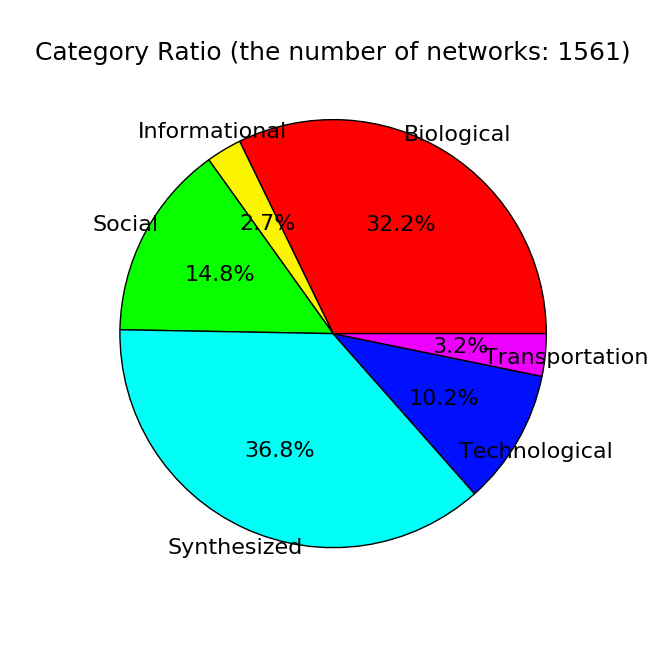
\includegraphics[width=\linewidth]{figs/category_ratio.png}
\caption{}\label{domain_ratio}
\end{subfigure}\hspace*{\fill}
\begin{subfigure}{0.45\textwidth}
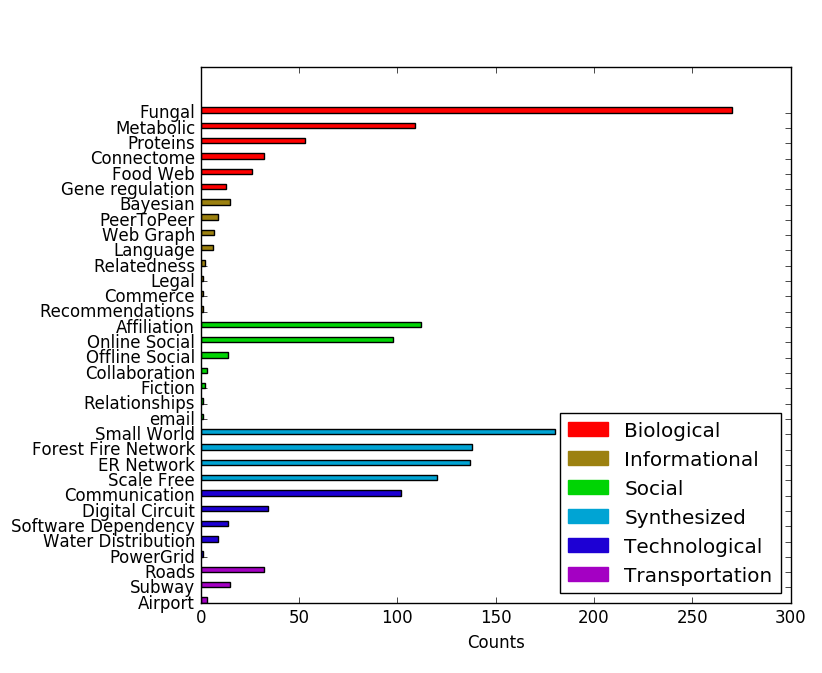
\includegraphics[width=\linewidth]{figs/subdomain_dist.png}
\caption{}\label{sub_dist}
\end{subfigure}\hspace*{\fill}

\caption{(a): The categorical ratio of network domains. (b):  Count distribution of network sub-domains. Sub-domains of the same network domain are grouped together having the same color in the figure. Color code from top: Biological, Informational, Social, Synthesized, Technological and Transportation.} \label{category_dist}.
\end{figure}


\newpage
	\begin{longtable}{| l | l | p{9cm} |}
	\caption{Network sub-domains and their descriptions.} \label{tab:subdomain}\\
	
	%header for the first page%
	\hline
 	Sub-domain & Domain& Description \\ \hline \hline
	 \endfirsthead
	 % header for after the first page
	 \multicolumn{3}{l}{\small\it Continued}\\ \hline
	 Sub-domain & Domain& Description \\ \hline \hline
 	\endhead
      %Sub-domain & Domain & Description  \\ \hline \hline
      Fungal &  Biological & Network of mycelial growth patterns of fungus or slime mold. Nodes are located at hyphal tips, branch points, and anastomoses. Edges represent cords.\\  %\hline
      Metabolic &  Biological & Network of chemical reactions of metabolism in a cell.\\  %\hline
      Proteins &  Biological & Physical contacts of proteins in a cell or in a living organism.\\  %\hline
      Connectome &  Biological & Network of neural connection in the brain at either the level of neuron or the level of anatomical region.\\  %\hline
      Food Web &  Biological & The relationships of predator-prey in terrestrial or aquatic animal kingdoms.\\  %\hline
      Gene regulation &  Biological & The interactions of molecular regulators that govern the gene expression.\\ % \hline
      Bayesian & Informational & Probabilistic model that contains a directed-acyclic-graph(DAG) in which nodes represent random variables and edges represent conditional dependence among these random variables.\\  %\hline
      PeerToPeer &  Informational & A kind of computer networks in which peers (computers) are equally privileged in the network for sharing files.\\ % \hline
      Web Graph &  Informational & Network of World-Wide-Web. Nodes represent web pages and edges represent hyper-links among web sites. \\  %\hline
      Language &  Informational & Networks of word adjacency and word association that are extracted from books.\\  \hline
      Relatedness &  Informational & Networks of relatedness, such as similarities among book purchased on online retailers. \\ % \hline
      Legal &  Informational & Network of legal citations. Nodes represent majority opinions written by the Supreme Court of the United States and edges represent citation.\\ % \hline
      Commerce &  Informational & Network of co-purchasing items on websites.\\  %\hline
      Recommendations &  Informational & Network of books, where edges represent the frequency that a pair of nodes (books) is co-purchased together.\\  %\hline
      Affiliation &  Social & Network of cooperate boards and the directors that sit on them. Networks in this sub-domain are one-mode projected onto individuals.\\  %\hline
      Online Social &  Social & Network of friendship online, such as Facebook.\\  %\hline
      Offline Social &  Social & Network of friendship or some sort of inter-personal relationships offline.\\  %\hline
      Collaboration &  Social & Network of collaborations among people. This sub-domain includes collaboration of scientific papers, music, etc.\\  %hline
      Fiction &  Social & Co-appearance network of fictional characters from books.\\  %\hline
      Relationships &  Social & Network of social relationship among managers from tech companies, Florentine families during the Italian Renaissance, etc.\\ % \hline
      Email &  Social & Network of emails.\\ % \hline
      Small World &  Synthesized & Networks generated by Watt-Strogatz model.\\  \hline
      Forest Fire Network &  Synthesized & Networks generated by a Forest Fire Model proposed by Leskovec \textit{et al.} \\  %\hline
      ER Network &  Synthesized & Erd\H{o}s-R\'enyi random network. \\  % \hline
      Scale Free &  Synthesized & Networks generated by Barab\'asi-Albert model.\\  %\hline
      Communication &  Technological & Network of autonomous systems (the Internet).\\  %\hline
      Digital Circuit &  Technological & Networks of logical gates connected by wirings.\\ % \hline
      Software Dependency &  Technological & Networks in which nodes represent either class, function or package and edges correspond to dependencies.\\  %\hline
      Water Distribution &  Technological & Network of piping and junctions for water distribution system.\\ % \hline
      Power Grid &  Technological & Network of power grid in which nodes correspond to transforms or power relay points and edges represent power lines.\\ % \hline
      Roads &  Transportation & Network of roads where nodes are intersections and edges are roads.\\ % \hline
      Subway &  Transportation & Subway networks of major cities around the world.\\ % \hline
      Airport &  Transportation & Network of airports that are connected by flights between the airports.\\  \hline
           
\end{longtable}
